\addtocontents{toc}{\protect\setcounter{tocdepth}{1}}
\chapter[Anexo: Planificación Inicial]{ANEXO: Planificación Inicial del Proyecto}

La planificación abarca 16 semanas de trabajo. Las primeras cuatro se dedican al
levantamiento de información con Enfermería, al análisis y al diseño, y las doce
restantes a la construcción en tres sprints. Las pruebas acompañan a cada sprint
y la documentación se elabora durante todo el proyecto. Al cierre de cada sprint
se revisa una versión instalable con la contraparte, marcada con un rombo en la
Figura~\ref{fig:gantt}.

\begin{figure}[H]
\centering
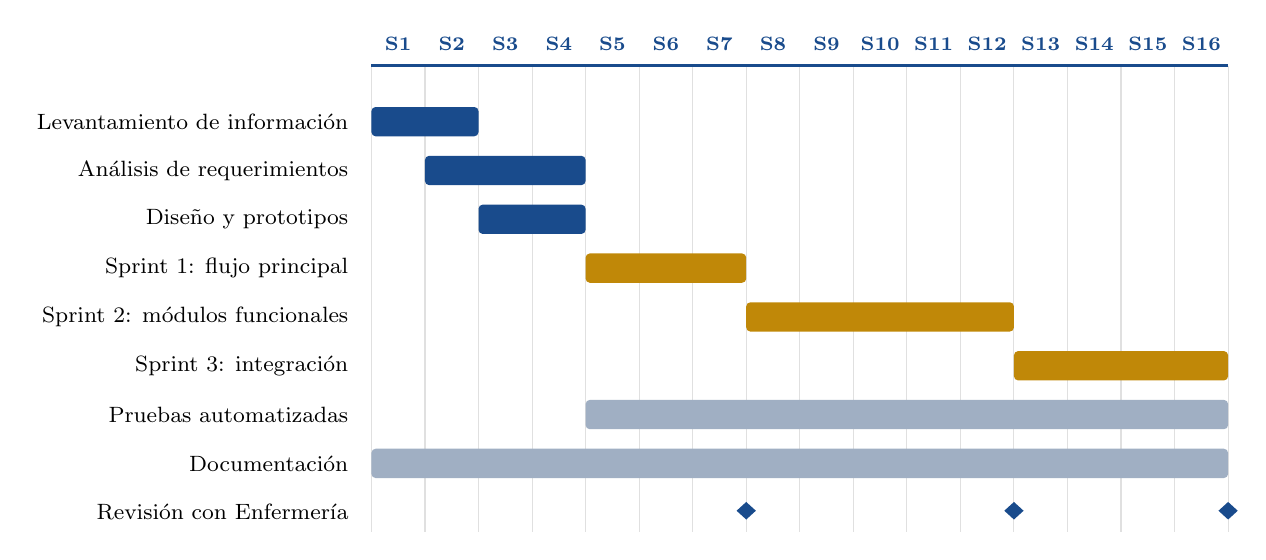
\begin{tikzpicture}[x=0.68cm, y=0.62cm, font=\footnotesize]
  \definecolor{ganttfase}{RGB}{25,75,140}
  \definecolor{ganttsprint}{RGB}{192,136,8}
  \definecolor{ganttsuave}{RGB}{160,175,195}
  % Cabecera de semanas
  \foreach \s in {1,...,16} {
    \node[font=\scriptsize\bfseries, text=ganttfase] at (\s-0.5, 0.7) {S\s};
    \draw[black!12] (\s,0.25) -- (\s,-9.3);
  }
  \draw[black!12] (0,0.25) -- (0,-9.3);
  \draw[ganttfase, thick] (0,0.25) -- (16,0.25);
  % Actividades: nombre, inicio, fin, color, fila
  \foreach \nombre/\ini/\fin/\col/\fila in {
      Levantamiento de información/0/2/ganttfase/1,
      Análisis de requerimientos/1/4/ganttfase/2,
      Diseño y prototipos/2/4/ganttfase/3,
      Sprint 1: flujo principal/4/7/ganttsprint/4,
      Sprint 2: módulos funcionales/7/12/ganttsprint/5,
      Sprint 3: integración/12/16/ganttsprint/6,
      Pruebas automatizadas/4/16/ganttsuave/7,
      Documentación/0/16/ganttsuave/8} {
    \node[anchor=east, align=right] at (-0.25,-\fila+0.1) {\nombre};
    \fill[\col, rounded corners=1.5pt] (\ini,-\fila-0.2) rectangle (\fin,-\fila+0.4);
  }
  % Hitos de revisión con Enfermería
  \node[anchor=east] at (-0.25,-8.9) {Revisión con Enfermería};
  \foreach \h in {7,12,16}
    \fill[ganttfase] (\h,-9.05) -- ++(0.18,0.18) -- ++(-0.18,0.18) -- ++(-0.18,-0.18) -- cycle;
\end{tikzpicture}
\caption{Carta Gantt del proyecto por semanas.}
\label{fig:gantt}
\end{figure}

Los sprints se ejecutan entre el 26 de agosto y el 13 de noviembre de 2026. El
sprint~1 cubre el flujo principal (HU-01 a HU-07 y HU-09 a HU-11), el sprint~2
la rutina del cuidador (HU-08 y HU-12 a HU-22) y el sprint~3 los aspectos
transversales (HU-24 a HU-27).

\section[Estimación Inicial de Tamaño]{Estimación inicial de tamaño}

El tamaño del software se estima con la técnica de puntos de caso de uso
\citep{pressman_2010}, a partir de los doce casos de uso del capítulo de
análisis.

\subsection*{Peso de los actores}

El cuidador principal interactúa mediante una interfaz gráfica, por lo que se
clasifica como actor complejo, con peso~3. La API del servidor de OnCuidar (con su
servicio de correo por SMTP) interactúa mediante un protocolo definido y se
clasifica como actor simple, con peso~1. Al reemplazar la plataforma externa
por el servidor propio la clasificación no cambia, de modo que el peso de los
actores sin ajustar sigue siendo UAW~=~3~+~1~=~4, y con él UUCP~=~124 y
UCP~$\approx$~129.

\subsection*{Peso de los casos de uso}

Cada caso de uso se clasifica según su número de transacciones. Los simples,
con hasta tres transacciones, pesan~5. Los medios, de cuatro a siete, pesan~10.
Los complejos, con más de siete, pesan~15.

\begin{table}[H]
\centering
\small
\tablazebra
\caption{Clasificación de los casos de uso.}
\label{tab:ucp-uucw}
\begin{tabularx}{\textwidth}{P{0.45}P{1.55}P{0.60}P{0.40}}
\toprule
\filaencabezado \encab{CU} & \encab{Nombre} & \encab{Complejidad} & \encab{Peso} \\
\midrule
CU-01 & Crear cuenta & Media & 10 \\
CU-02 & Iniciar sesión & Simple & 5 \\
CU-03 & Gestionar perfil del cuidador & Media & 10 \\
CU-04 & Gestionar pacientes & Compleja & 15 \\
CU-05 & Consultar panel principal & Simple & 5 \\
CU-06 & Registrar valoración clínica & Compleja & 15 \\
CU-07 & Consultar historial & Media & 10 \\
CU-08 & Exportar historial & Media & 10 \\
CU-09 & Consultar asistente de orientación & Media & 10 \\
CU-10 & Consultar preguntas frecuentes & Simple & 5 \\
CU-11 & Consultar biblioteca educativa & Compleja & 15 \\
CU-12 & Gestionar recordatorios & Media & 10 \\
\midrule
\filatotal \textbf{UUCW} & & & \textbf{120} \\
\bottomrule
\end{tabularx}
\end{table}

\subsection*{Cálculo de los puntos de caso de uso}

\begin{itemize}
    \item Puntos sin ajustar: UUCP = UUCW + UAW = 120 + 4 = 124.
    \item Factor de complejidad técnica, con una suma ponderada de 30:
    TCF = 0,6 + 0,01 × 30 = 0,90.
    \item Factor de ambiente, con una suma ponderada de 8:
    EF = 1,4 -- 0,03 × 8 = 1,16.
    \item Puntos ajustados: UCP = 124 × 0,90 × 1,16 $\approx$ 129.
\end{itemize}

Con el factor de 20 horas por UCP propuesto por Karner, el esfuerzo estimado
alcanza unas 2.580 horas. Como el presupuesto del proyecto es de 480 horas, esta
estimación fundamenta la decisión de acotar el alcance a un prototipo TRL~3 y
de priorizar el backlog en tres sprints.

\section[Contabilización Final de Tamaño]{Contabilización final del tamaño del software}

El tamaño se contabiliza sobre el repositorio, contando todas las líneas de los
archivos propios, sin incluir código generado ni paquetes externos. La
Tabla~\ref{tab:loc} conserva la medición histórica al cierre del sprint~2 e
incorpora la medición al cierre del proyecto, posterior a la migración al
servidor propio.

\begin{table}[H]
\centering
\small
\tablazebra
\caption{Tamaño del software al cierre del sprint 2 y al cierre del proyecto.}
\label{tab:loc}
\begin{tabularx}{\textwidth}{P{1.30}P{0.35}P{0.70}P{0.65}}
\toprule
\filaencabezado \encab{Componente} & \encab{Archivos} & \encab{Líneas totales} & \encab{Líneas no vacías} \\
\midrule
Código de la aplicación (lib/) al cierre del sprint~2 & 157 & 23.222 & 21.791 \\
Pruebas automatizadas (test/) al cierre del sprint~2 & 53 & 13.003 & 11.591 \\
\midrule
\multicolumn{4}{@{}l}{\itshape Al cierre del proyecto} \\
Código de la aplicación (lib/) & 188 & 27.413 & 25.602 \\
Pruebas de la aplicación (test/) & 37 & 4.664 & 4.095 \\
Código del backend (Node.js) & 16 & 1.483 & 1.346 \\
Pruebas del backend (tests/) & 6 & 665 & 597 \\
\bottomrule
\end{tabularx}
\end{table}

La relación entre el tamaño estimado y el código construido es de unas 180
líneas por UCP, con un esfuerzo planificado de 3,7 horas por UCP. La comparación
con las horas reales por fase se completará al cierre del sprint~3.
